
\documentclass[aspectratio=169,xcolor=dvipsnames]{beamer}
%\usetheme{SimplePlus}
\usepackage{hyperref}
\usepackage{graphicx} % Allows including images
\usepackage{booktabs} % Allows the use of \toprule, \midrule and \bottomrule in tables
\setbeamercolor{frametitle}{bg=white,fg=black}
\setbeamercolor{item}{bg=white,fg=black}
%\setbeameroption{show notes}

%----------------------------------------------------------------------------------------
%	TITLE PAGE
%----------------------------------------------------------------------------------------

\title[permas]{Person og Maskinsikkerhet} % The short title appears at the bottom of every slide, the full title is only on the title page
%\subtitle{Subtitle}

\author[Fred-Olav] {Fred-Olav Mosdal}

\institute[Gand VGS] % Your institution as it will appear on the bottom of every slide, may be shorthand to save space
{
    Gand VGS \\
    VG3 Automasjon }
\date{\today} % Date, can be changed to a custom date


%----------------------------------------------------------------------------------------
%	PRESENTATION SLIDES
%----------------------------------------------------------------------------------------

\begin{document}

\begin{frame}
	\frametitle{Personsikkerhet}
	\begin{columns}
		\begin{column}{0.5\textwidth}
			Automatikere jobber i miljøer med mange farer, det kan være:
		\begin{itemize}
			\item høye trykk
			\item høye temperaturer
			\item spenningsatte anlegg
			\item maskiner
			\item mekaniske prosesskomponeneter
			\item roboter
		\end{itemize}	
		\end{column}

		\begin{column}{0.5\textheight}
	$$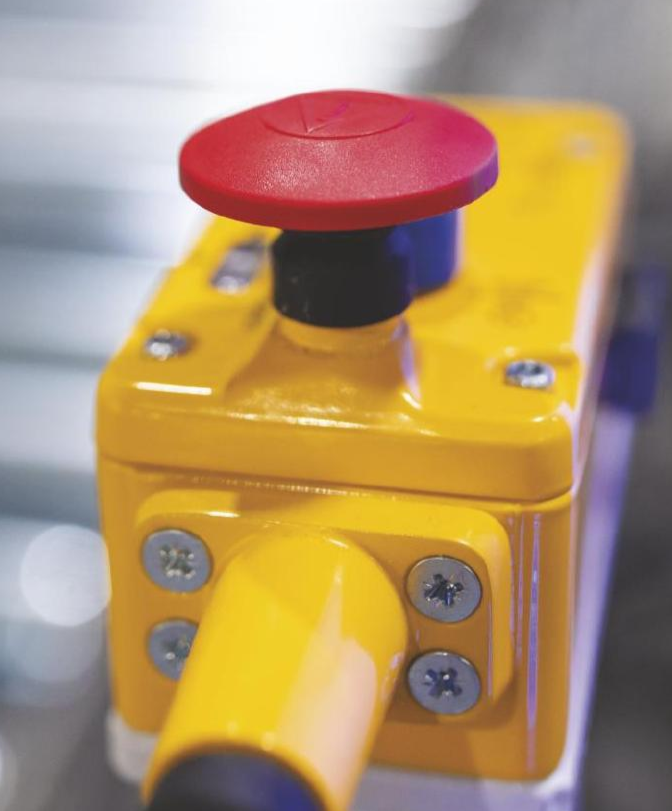
\includegraphics[height=0.8\textheight]{../output/nogpl/pPerMasSik01.png}$$
		\end{column}
	\end{columns}
\end{frame}
\begin{frame}
	\frametitle{Systematisk sikkerhetsarbeid}
	Alle virksomheter skal jobbe systematisk med sikkerhet.
	\vskip 10pt
	Det jobbes på tra nivåer:

	\begin{itemize}
		\item Forebyggende arbeid: Hvordan sikrer vi oss mot uønskede situasjoner?
		\item Handling: Hva gjør vi dersom det oppstår en nødssituasjon?
		\item Etterarbeid: Hva gjør vi etter en uventet og kritisk hendelse?
	\end{itemize}

\end{frame}


\begin{frame}
	\frametitle{Sikkerhetsbarierer}
	\begin{columns}
		\begin{column}{0.5\textwidth}
Det er mange barrierer som kan indre at en uønsket hendelse oppstår. 
\vskip 10pt
Hvor hver barriere som ikke virker øker sannsynligheten for en uønsket hendelse
			
		\end{column}

		\begin{column}{0.5\textwidth}
	$$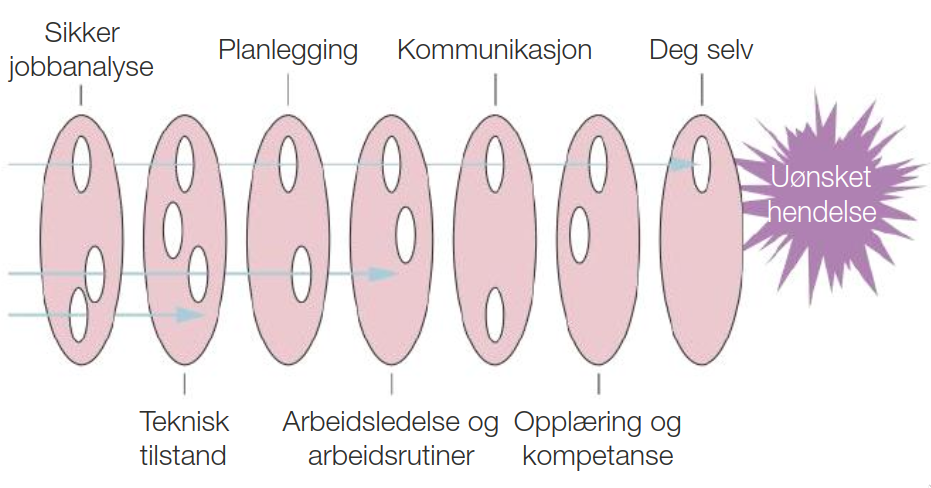
\includegraphics[width=1\textwidth]{../output/nogpl/pPerMasSik02.png}$$
		\end{column}
	\end{columns}
\end{frame}

\begin{frame}
	\frametitle{Sikker-jobb-analyse (SJA)}
	\begin{columns}
		\begin{column}{0.5\textwidth}
I industrien er det vanlig å gjøre en SJA før arbeidet starter. 
			
		\end{column}


		\begin{column}{0.5\textwidth}
	$$\includegraphics[width=1\textwidth]{../output/nogpl/SJA-skjema.png}$$
		\end{column}
	\end{columns}
\end{frame}
\begin{frame}
	\frametitle{Hva koster en ulykke?}	
\begin{itemize}
	\item Det dør ca. 30 personer pr år i arbeidsulykker
	\item Sammfunnskostnaden med sykdom og skader er 30 milliarder pr år. 
	\item Disse kostnadene kan reduseres ved å sette inn prevantive tilkak 
\end{itemize}



\end{frame}
\begin{frame}
	\frametitle{HMS-plan}
	\begin{columns}
		\begin{column}{0.5\textwidth}
	Alle bedrifter skal ha en HMS-plan. Her vises et typisk eksempel på en HMS-plan for et firma der automatikkere jobber.  
	\vskip 10pt
	HMS-planen må gjennomgås jevnlig. 
		\end{column}


		\begin{column}{0.5\textwidth}
	$$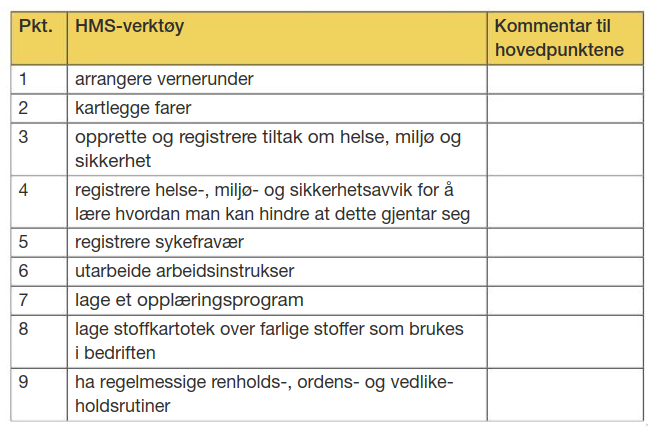
\includegraphics[width=1\textwidth]{../output/nogpl/pPerMasSik03.png}$$
		\end{column}
	\end{columns}
\end{frame}

\begin{frame}
	\frametitle{Kjemikalier og gasser}
	\begin{columns}
		\begin{column}{0.5\textwidth}
	Kjemikalier brukes mange plasser i industrien. Noen av disse stoffene er det vi kaller farlige kjemikalier. Det vil si at de kan medføre helse-, miljø-, brann- eller eksplosjonsfare. 
	\vskip 10 pt. 
	En bedrift skal ha et stoffkartotek over farlige kjemikalier som de bruker. 
			
		\end{column}

		\begin{column}{0.5\textwidth}
	$$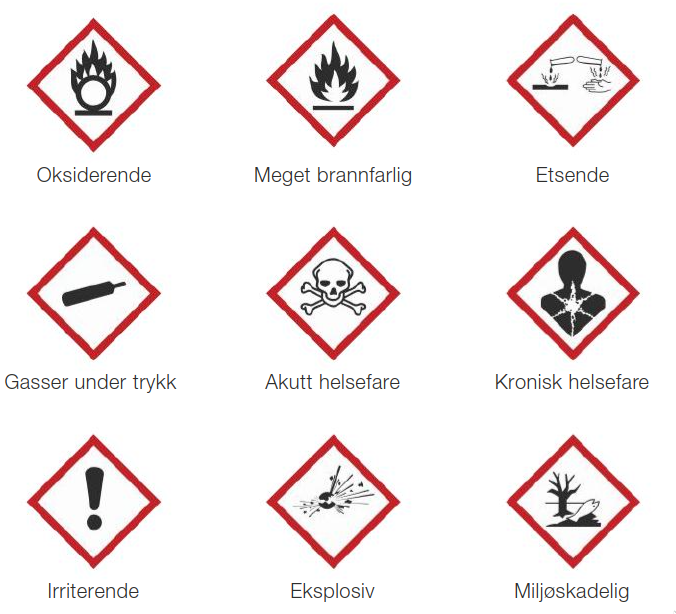
\includegraphics[width=1\textwidth]{../output/nogpl/pPerMasSik04.png}$$
		\end{column}
	\end{columns}
\end{frame}

\begin{frame}
	\frametitle{Løsemidler}
	\begin{columns}
		\begin{column}{0.5\textwidth}

			Løsemidler brukes i industrien for å løse opp andre stoffer, det eneste løsemiddelet kroppen tåler er vann. Vi kan skades av løsemiddler ved å:
			\begin{itemize}
				\item puste inn løsemiddeldamp, som tas opp i blodomløpet og lagres i fettvev. 
				\item ekspondering på huden, som tas opp igjennom hudensceller. 
			\end{itemize}


		\end{column}

		\begin{column}{0.5\textwidth}
	$$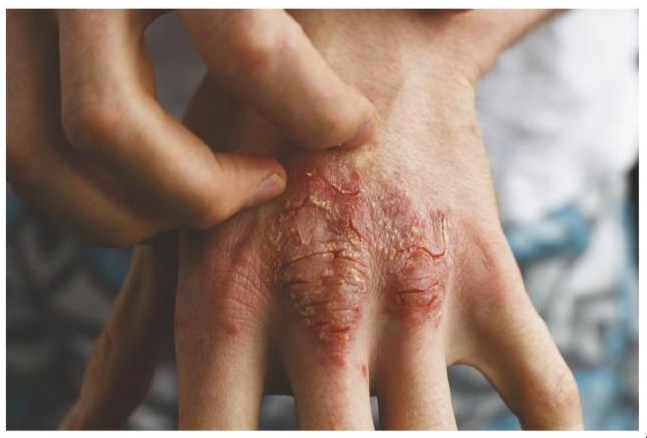
\includegraphics[width=1\textwidth]{../output/nogpl/pPerMasSik05.png}$$
		\end{column}
	\end{columns}
\end{frame}

\begin{frame}
	\frametitle{Løsmiddelskader på i kroppen}
	\begin{columns}
		\begin{column}{0.5\textwidth}
Hjernen og nervesystemet er utsatt for løsemiddelskader. En kan få symptomer som: 
	\begin{itemize}
		\item tretthet
		\item hodepine
		\item svimmelhet
		\item beruselse
		\item kvalme
	\end{itemize}
		\end{column}

		\begin{column}{0.5\textwidth}
	$$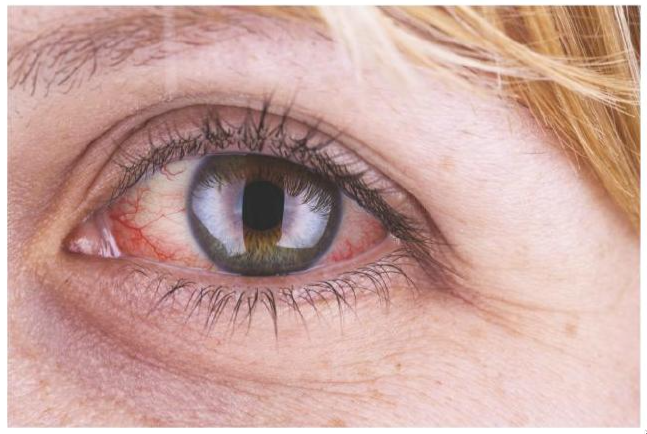
\includegraphics[width=1\textwidth]{../output/nogpl/pPerMasSik06.png}$$
		\end{column}
	\end{columns}
\end{frame}

\begin{frame}
	\frametitle{Bruk verneutstyr ved bruk av løsemidler}
	\begin{columns}
		\begin{column}{0.5\textwidth}
			
		\end{column}

		\begin{column}{0.5\textwidth}
	$$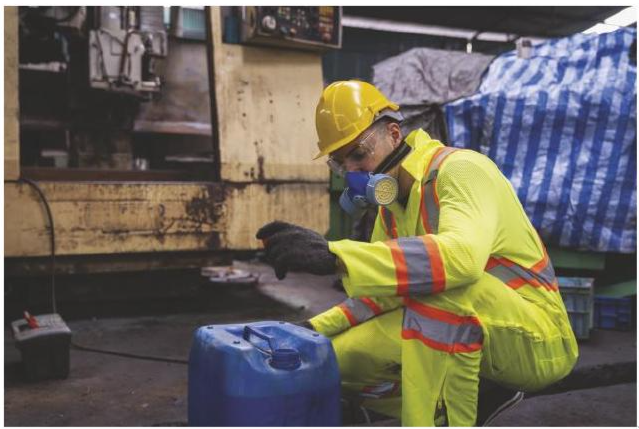
\includegraphics[width=1\textwidth]{../output/nogpl/pPerMasSik07.png}$$
		\end{column}
	\end{columns}
\end{frame}

\begin{frame}
	\frametitle{Arbeid i høyden}
	\begin{columns}
		\begin{column}{0.5\textwidth}
I fabrikker og på prosessnalegg må det av og til monteres utstyr høyt over gulvet. Når vi må jobbe på dette utstyret kalles det arbeid i høyden. 			
\begin{itemize}
	\item det er krav til tiltak ved arbeid over 1m over bakken. 
	\item over 2 meter er det krav til rekkverk eller personlig fallsikkrings utstyr. 
\end{itemize}
		\end{column}

		\begin{column}{0.5\textwidth}
	$$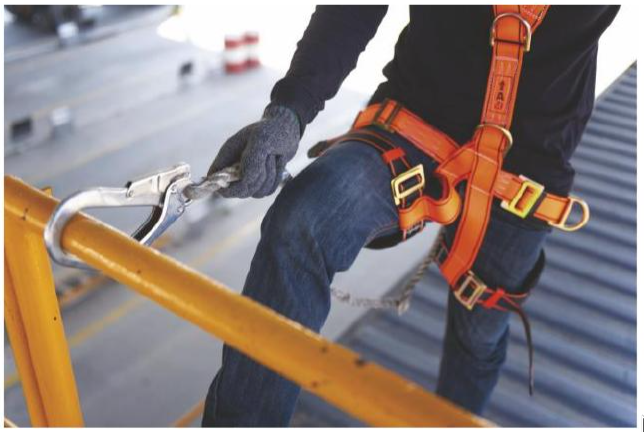
\includegraphics[width=1\textwidth]{../output/nogpl/pPerMasSik08.png}$$
		\end{column}
	\end{columns}
\end{frame}

\begin{frame}
	\frametitle{Tittel}
	\begin{columns}
		\begin{column}{0.5\textwidth}
tekst
			
		\end{column}

		\begin{column}{0.5\textwidth}
	$$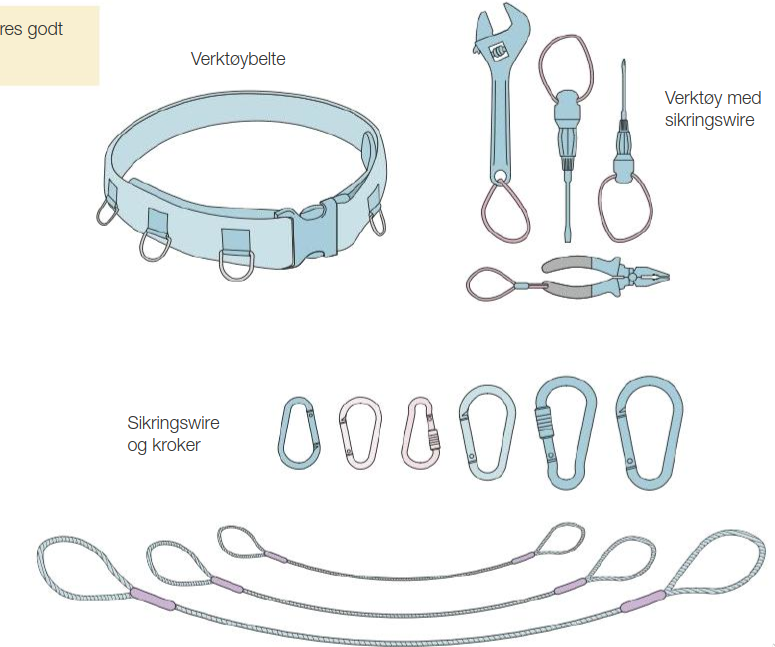
\includegraphics[width=1\textwidth]{../output/nogpl/pPerMasSik09.png}$$
		\end{column}
	\end{columns}
\end{frame}

\begin{frame}
	\frametitle{Tittel}
	\begin{columns}
		\begin{column}{0.5\textwidth}
tekst
			
		\end{column}

		\begin{column}{0.5\textwidth}
	$$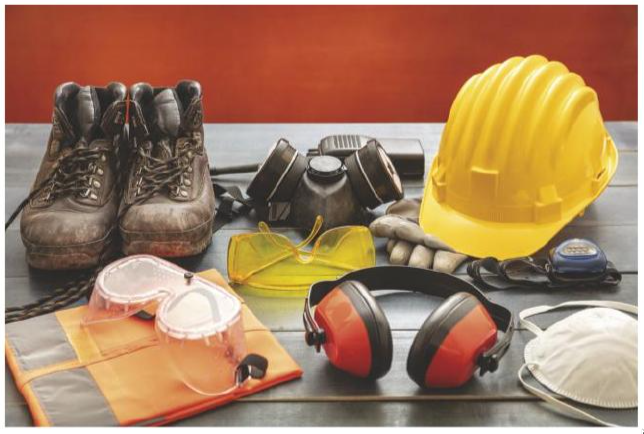
\includegraphics[width=1\textwidth]{../output/nogpl/pPerMasSik10.png}$$
		\end{column}
	\end{columns}
\end{frame}

\begin{frame}
	\frametitle{Tittel}
	\begin{columns}
		\begin{column}{0.5\textwidth}
tekst
			
		\end{column}

		\begin{column}{0.5\textwidth}
	$$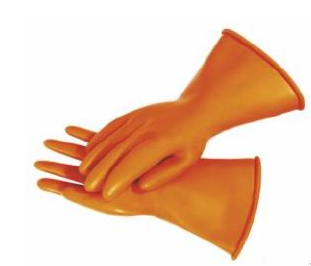
\includegraphics[width=1\textwidth]{../output/nogpl/pPerMasSik11.png}$$
		\end{column}
	\end{columns}
\end{frame}

\begin{frame}
	\frametitle{Tittel}
	\begin{columns}
		\begin{column}{0.5\textwidth}
tekst
			
		\end{column}

		\begin{column}{0.5\textwidth}
	$$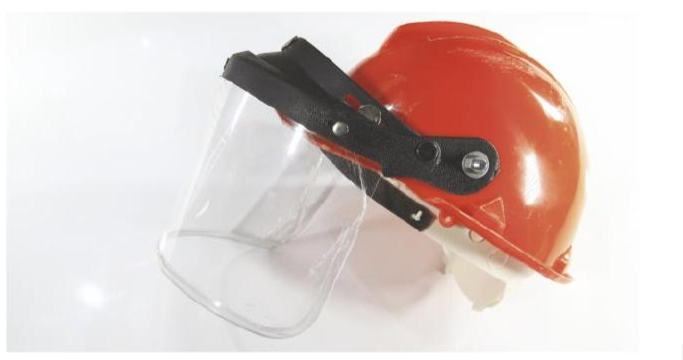
\includegraphics[width=1\textwidth]{../output/nogpl/pPerMasSik12.png}$$
		\end{column}
	\end{columns}
\end{frame}

\begin{frame}
	\frametitle{Tittel}
	\begin{columns}
		\begin{column}{0.5\textwidth}
tekst
			
		\end{column}

		\begin{column}{0.5\textwidth}
	$$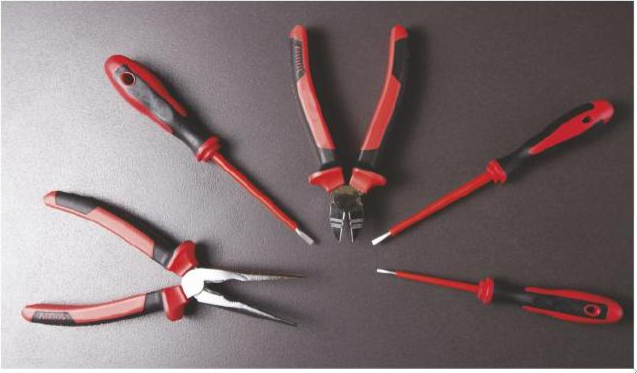
\includegraphics[width=1\textwidth]{../output/nogpl/pPerMasSik13.png}$$
		\end{column}
	\end{columns}
\end{frame}

\begin{frame}
	\frametitle{Tittel}
	\begin{columns}
		\begin{column}{0.5\textwidth}
tekst
			
		\end{column}

		\begin{column}{0.5\textwidth}
	$$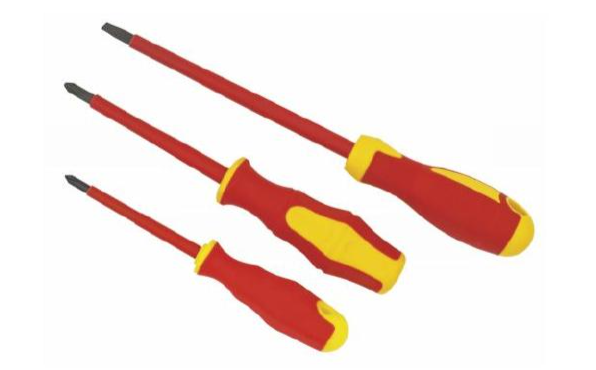
\includegraphics[width=1\textwidth]{../output/nogpl/pPerMasSik14.png}$$
		\end{column}
	\end{columns}
\end{frame}

\begin{frame}
	\frametitle{Tittel}
	\begin{columns}
		\begin{column}{0.5\textwidth}
tekst
			
		\end{column}

		\begin{column}{0.5\textwidth}
	$$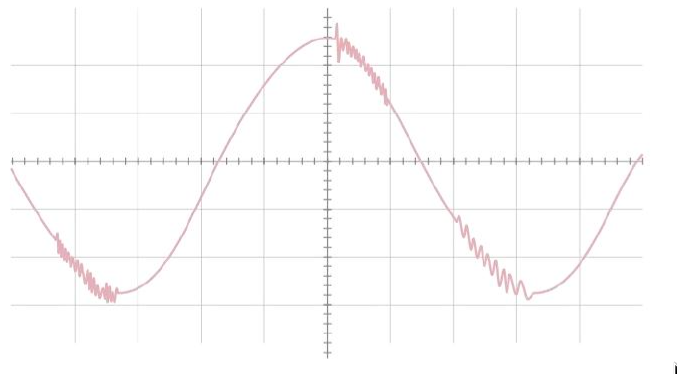
\includegraphics[width=1\textwidth]{../output/nogpl/pPerMasSik15.png}$$
		\end{column}
	\end{columns}
\end{frame}

\begin{frame}
	\frametitle{Tittel}
	\begin{columns}
		\begin{column}{0.5\textwidth}
tekst
			
		\end{column}

		\begin{column}{0.5\textwidth}
	$$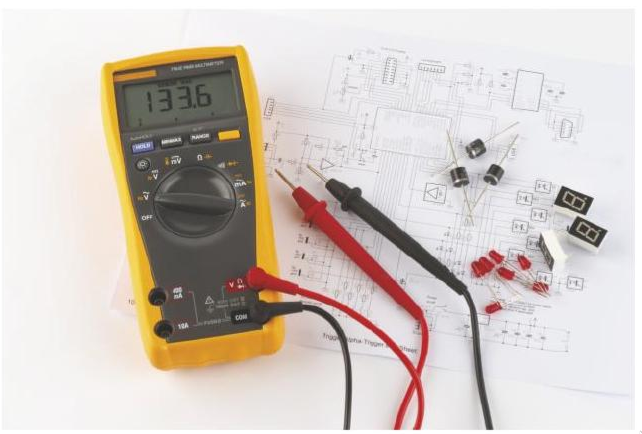
\includegraphics[width=1\textwidth]{../output/nogpl/pPerMasSik16.png}$$
		\end{column}
	\end{columns}
\end{frame}

\begin{frame}
	\frametitle{Tittel}
	\begin{columns}
		\begin{column}{0.5\textwidth}
tekst
			
		\end{column}

		\begin{column}{0.5\textwidth}
	$$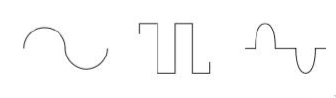
\includegraphics[width=1\textwidth]{../output/nogpl/pPerMasSik17.png}$$
		\end{column}
	\end{columns}
\end{frame}

\begin{frame}
	\frametitle{Tittel}
	\begin{columns}
		\begin{column}{0.5\textwidth}
tekst
			
		\end{column}

		\begin{column}{0.5\textwidth}
	$$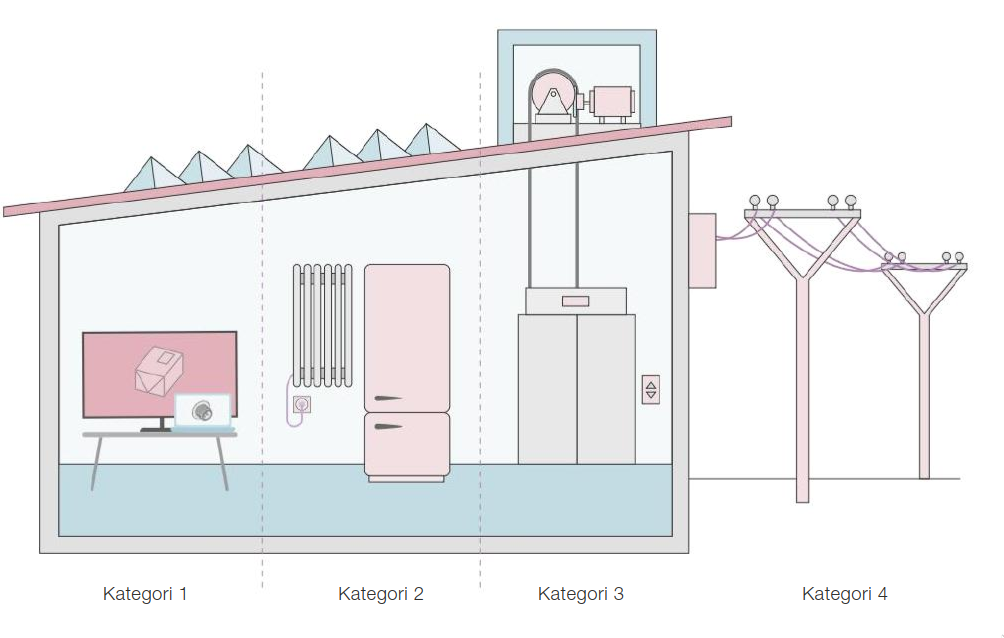
\includegraphics[width=1\textwidth]{../output/nogpl/pPerMasSik18.png}$$
		\end{column}
	\end{columns}
\end{frame}

\begin{frame}
	\frametitle{Tittel}
	\begin{columns}
		\begin{column}{0.5\textwidth}
tekst
			
		\end{column}

		\begin{column}{0.5\textwidth}
	$$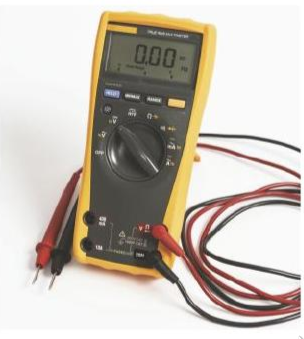
\includegraphics[width=1\textwidth]{../output/nogpl/pPerMasSik19.png}$$
		\end{column}
	\end{columns}
\end{frame}

\begin{frame}
	\frametitle{Tittel}
	\begin{columns}
		\begin{column}{0.5\textwidth}
tekst
			
		\end{column}

		\begin{column}{0.5\textwidth}
	$$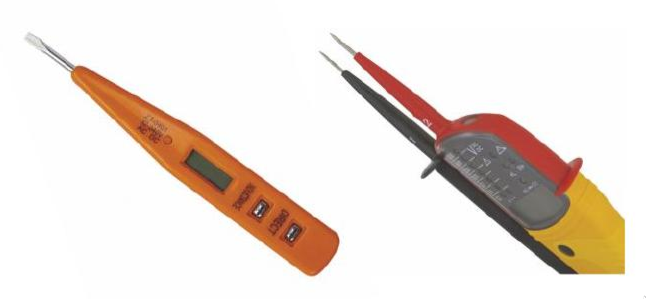
\includegraphics[width=1\textwidth]{../output/nogpl/pPerMasSik20.png}$$
		\end{column}
	\end{columns}
\end{frame}

\begin{frame}
	\frametitle{Tittel}
	\begin{columns}
		\begin{column}{0.5\textwidth}
tekst
			
		\end{column}

		\begin{column}{0.5\textwidth}
	$$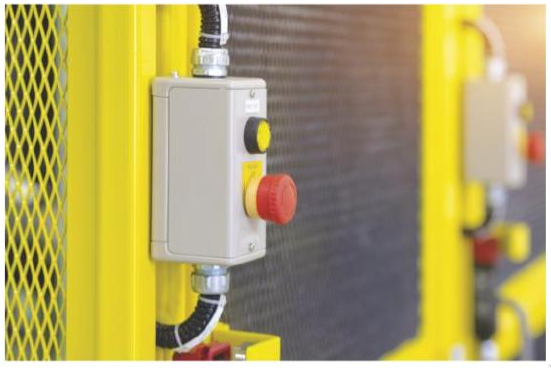
\includegraphics[width=1\textwidth]{../output/nogpl/pPerMasSik21.png}$$
		\end{column}
	\end{columns}
\end{frame}

\begin{frame}
	\frametitle{Tittel}
	\begin{columns}
		\begin{column}{0.5\textwidth}
tekst
			
		\end{column}

		\begin{column}{0.5\textwidth}
	$$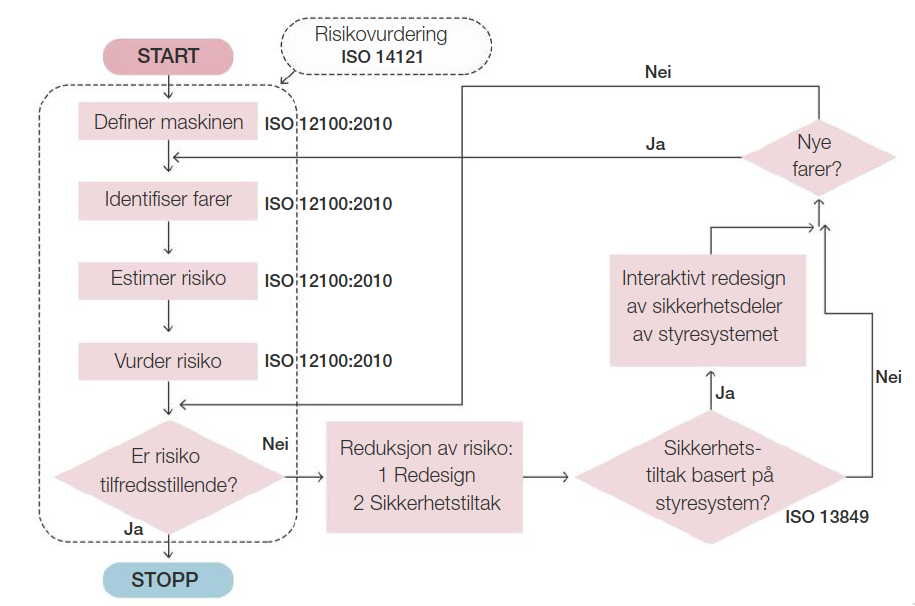
\includegraphics[width=1\textwidth]{../output/nogpl/pPerMasSik22.png}$$
		\end{column}
	\end{columns}
\end{frame}

\begin{frame}
	\frametitle{Tittel}
	\begin{columns}
		\begin{column}{0.5\textwidth}
tekst
			
		\end{column}

		\begin{column}{0.5\textwidth}
	$$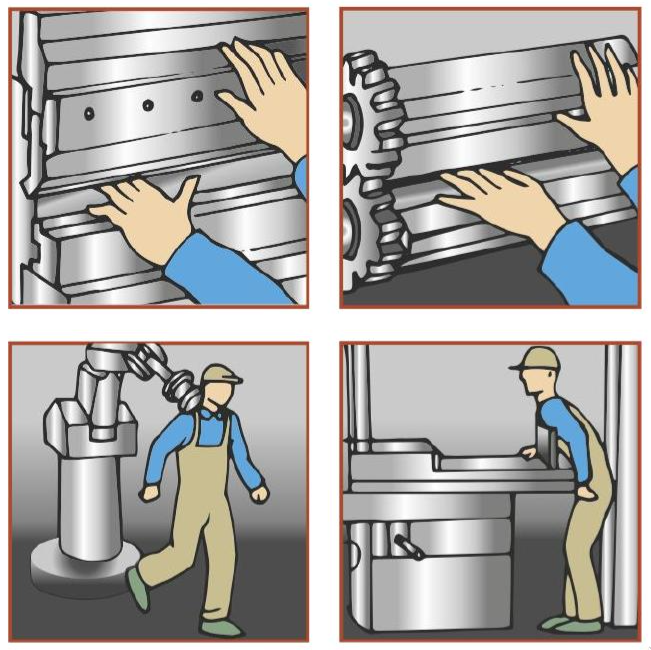
\includegraphics[width=1\textwidth]{../output/nogpl/pPerMasSik23.png}$$
		\end{column}
	\end{columns}
\end{frame}

\begin{frame}
	\frametitle{Tittel}
	\begin{columns}
		\begin{column}{0.5\textwidth}
tekst
			
		\end{column}

		\begin{column}{0.5\textwidth}
	$$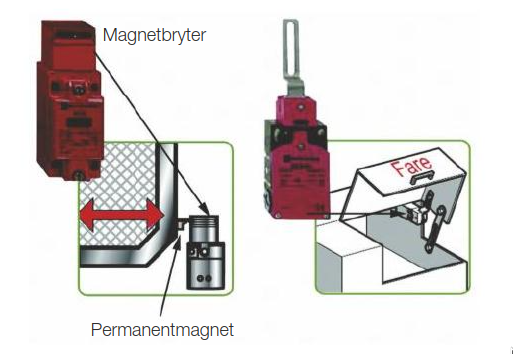
\includegraphics[width=1\textwidth]{../output/nogpl/pPerMasSik24.png}$$
		\end{column}
	\end{columns}
\end{frame}

\begin{frame}
	\frametitle{Tittel}
	\begin{columns}
		\begin{column}{0.5\textwidth}
tekst
			
		\end{column}

		\begin{column}{0.5\textwidth}
	$$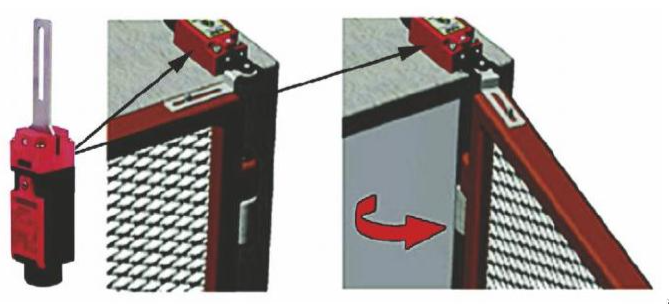
\includegraphics[width=1\textwidth]{../output/nogpl/pPerMasSik25.png}$$
		\end{column}
	\end{columns}
\end{frame}

\begin{frame}
	\frametitle{Tittel}
	\begin{columns}
		\begin{column}{0.5\textwidth}
tekst
			
		\end{column}

		\begin{column}{0.5\textwidth}
	$$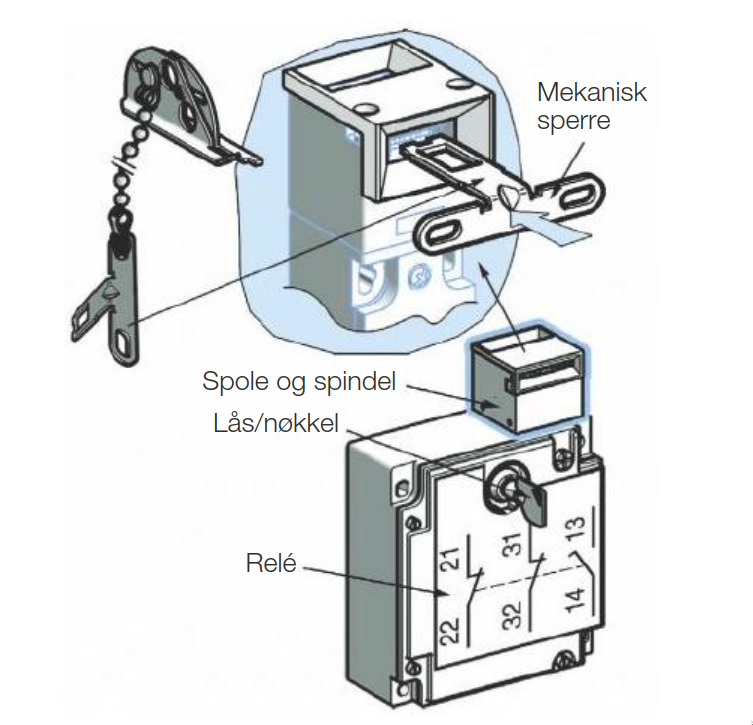
\includegraphics[width=1\textwidth]{../output/nogpl/pPerMasSik26.png}$$
		\end{column}
	\end{columns}
\end{frame}

\begin{frame}
	\frametitle{Maskinsikkerhet}
\end{frame}


\begin{frame}
	\frametitle{Introduksjon}
\begin{itemize}
	\item Hva er maskinsikkerhet?
		\note{Maskinsikkerhet handler om å sørge for at maskiner og utstyr er utformet, bygd og driftet på en måte som minimerer risikoen for ulykker og skader på personer og miljø. Maskinsikkerhet omfatter en rekke tiltak og teknologier, inkludert risikovurderinger, sikkerhetskomponenter, sikkerhetsfunksjoner i styringssystemet, utforming av maskinen og opplæring og vedlikehold av personalet som jobber med maskinen. Maskinsikkerhet er svært viktig for å beskytte arbeidstakere, forebygge tap av produksjon og økonomiske tap, samt for å unngå skade på miljøet og for å overholde lovgivning og forskrifter.}
	\item Hvorfor er det viktig?
\end{itemize}
\end{frame}
\begin{frame}
	\frametitle{Lover og regler}

\begin{itemize}
	\item Hva sier loven om maskinsikkerhet?
		\note{Loven om maskinsikkerhet varierer fra land til land, men de fleste land har lover og forskrifter som krever at maskiner og utstyr er utformet, bygd og driftet på en sikker måte som beskytter arbeidstakere og omgivelsene.

I EU er maskindirektivet (Directive 2006/42/EC) den viktigste loven for maskinsikkerhet. Denne direktivet stiller krav til at produsenter av maskiner og utstyr tar hensyn til sikkerheten til mennesker og miljøet når de utformer og bygger sine produkter. Direktivet krever at produsenter utfører risikovurderinger, dokumenterer sikkerhetskravene, og leverer maskinen med CE-merking og nødvendig dokumentasjon.

I USA er Occupational Safety and Health Administration (OSHA) en viktig organisasjon som regulerer maskinsikkerhet. OSHA har utviklet standarder for maskinsikkerhet som regulerer utforming, konstruksjon og bruk av maskiner og utstyr, og som krever risikovurderinger og implementering av nødvendige sikkerhetstiltak.

		I Norge er Arbeidstilsynet ansvarlig for å håndheve maskinforskriften som beskriver krav til utforming, konstruksjon og bruk av maskiner og utstyr. Maskinforskriften er basert på EUs maskindirektiv og stiller krav til CE-merking og dokumentasjon av risikovurderinger og sikkerhetstiltak.}
	\item Hvilke regler må følges?
		\note{I Norge er maskinforskriften en av de viktigste forskriftene som regulerer maskinsikkerhet. Denne forskriften er basert på EUs maskindirektiv og gjelder for alle som produserer, importerer, omsetter eller tar i bruk maskiner og tekniske hjelpemidler. Forskriften krever at maskiner og utstyr er utformet, bygd og driftet på en sikker måte som beskytter arbeidstakere og omgivelsene.

I tillegg til maskinforskriften finnes det andre relevante regler som også gjelder for maskinsikkerhet i Norge, blant annet:

Forskrift om utførelse av arbeid: Denne forskriften stiller krav til at arbeidsgiver skal sørge for at arbeidet blir utført på en slik måte at arbeidstakerne ikke utsettes for fare for liv eller helse.

Forskrift om verneombud og arbeidsmiljøutvalg: Denne forskriften stiller krav til at det skal velges verneombud på arbeidsplassen og at arbeidsmiljøutvalg skal opprettes dersom det er mer enn 50 ansatte.

Forskrift om bruk av arbeidsutstyr: Denne forskriften stiller krav til at arbeidsutstyr skal velges og brukes på en slik måte at det ikke medfører fare for liv og helse.

Forskrift om organisering, ledelse og medvirkning: Denne forskriften stiller krav til at arbeidsgiver skal sørge for at det foreligger systemer for å ivareta arbeidsmiljøet på arbeidsplassen.

		Det er viktig å merke seg at det kan være ulike krav avhengig av hvilken type maskin eller utstyr som brukes og hvilken sektor arbeidet foregår i, for eksempel industri, bygg- og anlegg eller landbruk. Derfor er det viktig å undersøke hvilke spesifikke regler som gjelder for den konkrete situasjonen.
De relevante normene for maskinforskriften i Norge er blant annet:

NS-EN ISO 12100:2010 - Sikkerhet for maskiner - Generelle krav til konstruksjon og risikovurdering
NS-EN ISO 13849-1:2016 - Sikkerhet for maskiner - Sikkerhetsrelaterte deler av kontrollsystemer - Del 1: Generelle prinsipper for utforming
NS-EN ISO 13850:2015 - Sikkerhet for maskiner - Nødstop - Prinsipper for utforming
NS-EN ISO 14121-1:2007 - Sikkerhet for maskiner - Risikovurdering - Del 1: Prinsipper
Disse normene gir retningslinjer for hvordan maskiner bør designes og konstrueres for å oppfylle sikkerhetskravene i maskinforskriften. De gir også veiledning for risikovurdering og utforming av sikkerhetsrelaterte deler av kontrollsystemer.

For elektrisk utstyr i maskiner, gjelder normen NS-EN 60204-1:2018 "Sikkerhet for maskiner - Elektrisk utstyr - Del 1: Generelle krav". Denne normen gir krav til elektrisk utstyr som brukes i maskiner, og gir retningslinjer for utforming av elektriske systemer og installasjoner som brukes i maskiner.

NS-EN 60204-1:2018 dekker temaer som isolasjon, jording, beskyttelse mot elektrisk støt, beskyttelse mot overstrøm og kortslutning, beskyttelse mot elektriske farer, krav til elektriske kontroller, samt merking og dokumentasjon av elektrisk utstyr.

Det er viktig å merke seg at overholdelse av normen NS-EN 60204-1:2018 ikke automatisk oppfyller kravene i maskindirektivet eller maskinforskriften, men den er likevel en viktig del av å oppfylle kravene til elektrisk sikkerhet i maskiner.
		}
\end{itemize}
\end{frame}
\begin{frame}
	\frametitle{Risikovurdering}


\begin{itemize}
	\item Hva er en risikovurdering?
		\note{n risikovurdering er en systematisk vurdering av risikoer knyttet til en gitt aktivitet, prosess eller situasjon. Formålet med en risikovurdering er å identifisere farer, evaluere risikoer og utvikle en plan for å redusere risikoene eller eliminere dem helt.

Risikovurderinger brukes ofte i industrielle og kommersielle settinger for å vurdere risikoene knyttet til produksjon, lagring og transport av farlige materialer, eller for å identifisere potensielle sikkerhetsrisikoer for arbeidere. Risikovurderinger kan også brukes i forbindelse med byggeprosjekter eller i forbindelse med utvikling av produkter eller tjenester.

En typisk risikovurdering innebærer å identifisere potensielle farer, vurdere sannsynligheten for at de vil oppstå, og evaluere konsekvensene hvis de faktisk oppstår. Deretter kan man identifisere tiltak for å redusere risikoen, og prioritere disse tiltakene basert på alvorlighetsgraden av risikoen.

		Risikovurderinger kan bidra til å identifisere potensielle farer og risikoer på forhånd, slik at man kan implementere tiltak for å redusere risikoen og beskytte arbeidere, samfunnet og miljøet.}
	\item Hvorfor er det viktig å gjøre en risikovurdering?
\end{itemize}
\end{frame}
\begin{frame}
	\frametitle{Sikkerhetskomponenter}


\begin{itemize}
	\item Hva er sikkerhetskomponenter?
		\note{Sikkerhetskomponenter er spesielle enheter som er utformet for å beskytte mennesker, miljøet og utstyret mot skade eller ulykker som kan oppstå som følge av maskinens drift eller feil. Disse enhetene kan brukes i ulike situasjoner for å minimere risikoen og sørge for at maskinen fungerer på en sikker måte.

Eksempler på sikkerhetskomponenter inkluderer:

Sikkerhetsbrytere: Disse er enheter som er installert for å bryte strømmen eller signalet som går til en maskin når det oppstår en feil, eller når en operatør utfører en bestemt handling.

Lysgitter: Dette er en serie med infrarøde lysstråler som plasseres rundt en maskin for å skape et usynlig gjerde. Hvis en person eller gjenstand kommer inn i dette området, vil maskinen stoppes umiddelbart.

Sikkerhetsscannere: Dette er enheter som kan skanne en bestemt del av maskinen og oppdage om noen kommer for nær, eller om det er en uvanlig bevegelse.

Sikkerhetsventiler: Disse er enheter som er installert for å beskytte mot overtrykk eller for høy temperatur i et system.

		Sikkerhetssensorer: Disse kan oppdage bevegelse, berøring eller tilstedeværelse av en person eller gjenstand i et bestemt område, og de kan utløse en alarm eller stoppe maskinen.}
	\item Eksempler på sikkerhetskomponenter (sensorer, brytere, lysgitter, sikkerhetsreleer)
\end{itemize}
\end{frame}
\begin{frame}
	\frametitle{Sikkerhetsfunksjoner i styringssystemet}


\begin{itemize}
	\item Hva er sikkerhetsfunksjoner i styringssystemet?
		\note{Sikkerhetsfunksjoner i et styringssystem er spesielle funksjoner som er designet for å oppdage farlige situasjoner og iverksette passende tiltak for å unngå eller redusere risikoen for personskader og skade på utstyr. Dette kan inkludere funksjoner som:

Nødstoppfunksjon: Dette er en funksjon som er utformet for å stoppe en maskin eller en prosess raskt når det oppstår en farlig situasjon, for eksempel en fare for personskade.

Sikkerhetsdører: Sikkerhetsdører er dører som er utformet for å forhindre at personer eller gjenstander kommer inn i farlige soner, som en maskin som er i gang.

Lysgitter: Lysgitter er sensorer som bruker en rekke lysstråler for å oppdage om en person eller gjenstand er til stede i en farlig sone.

Sikkerhetsbrytere: Sikkerhetsbrytere er spesielle brytere som er utformet for å registrere når en sikkerhetsdør åpnes eller lukkes, og sende en signal til styringssystemet for å stoppe eller starte maskinen.

Overvåking av hastighet og posisjon: Overvåking av hastighet og posisjon kan brukes til å oppdage om en maskin beveger seg unormalt raskt eller er ute av posisjon, og iverksette tiltak for å unngå farlige situasjoner.

		Sikkerhetsfunksjoner er viktige for å opprettholde et trygt arbeidsmiljø og redusere risikoen for personskader og skade på utstyr. De må velges og implementeres riktig for å oppfylle de spesifikke sikkerhetskravene til den aktuelle maskinen eller prosessen.}
	\item Eksempler på sikkerhetsfunksjoner (blokkering av farlige bevegelser, sikkerhetsbremsing, nødstoppsystemer)
\end{itemize}
\end{frame}
\begin{frame}
	\frametitle{Utforming av maskinen}


\begin{itemize}
	\item Hva betyr utforming av maskinen?
		\note{Utforming av maskinen kan ha stor påvirkning på risikonivået knyttet til maskinen. En maskin som er utformet på en sikker måte vil ha færre farlige situasjoner enn en maskin som er utformet på en usikker måte. Faktorer som kan påvirke risikoen knyttet til maskinens utforming inkluderer:

Tilgjengelighet til farlige deler: En maskin som har farlige deler som er lett tilgjengelig for operatøren kan øke risikoen for ulykker. Dette kan inkludere deler som beveger seg i høy hastighet eller deler som er varme og kan forårsake brannskader.

Bevegelse av deler: Hvis en maskin har deler som beveger seg i høy hastighet, kan det øke risikoen for ulykker. Dette kan inkludere bevegelige deler som kutteverktøy, transportbånd eller roterende aksler.

Utforming av kontroller: Hvis kontrollene på maskinen er vanskelige å bruke eller forstå, kan det øke risikoen for feilbetjening eller ulykker. Dette kan inkludere kontrollpaneler som er overfylte eller vanskelig å lese, eller knapper som er plassert på feil steder.

Materialer og konstruksjon: Hvis maskinen er konstruert av dårlige materialer eller har svake punkter i konstruksjonen, kan det øke risikoen for ulykker. Dette kan inkludere sveisede ledd som er svake eller sprekker, eller materialer som ikke tåler de påkjenningene som maskinen utsettes for.

Tilgjengelighet til verneutstyr: Hvis maskinen ikke har tilstrekkelig verneutstyr, som f.eks. sikkerhetsgjerder eller vernebriller, kan det øke risikoen for ulykker. Dette kan inkludere maskiner som mangler skjerming rundt farlige deler eller som ikke har tilstrekkelig belysning til å se farlige situasjoner.

		Det er derfor viktig å ta hensyn til alle disse faktorene når man designer og konstruerer maskiner, og å sørge for at maskinen overholder relevante sikkerhetsstandarder og -forskrifter.}
	\item Eksempler på utformingstiltak (skjerming av bevegelige deler, plassering av deler utenfor rekkevidde)
		\note{Monter skjermer og fysiske barrierer: Dette kan hindre at operatørene kommer i kontakt med farlige bevegelige deler eller prosesser.

Installer sikkerhetsbrytere: Monter brytere som deaktiverer maskinen dersom en skjerm eller en dør blir åpnet, eller hvis noen kommer for nær farlige bevegelige deler.

Monter nødstopp-knapper: Monter nødstopp-knapper på et tilgjengelig sted slik at operatører raskt kan stanse maskinen i en nødsituasjon.

Reduser hastigheten: Redusere hastigheten på bevegelige deler kan redusere risikoen for personskade.

Monter varslingssystemer: Installer varslingssystemer som lyd- eller lysalarmer for å varsle operatører om farlige situasjoner.

Bruk ergonomisk utforming: Sørg for at maskinen er ergonomisk utformet slik at operatørene kan jobbe effektivt og sikkert.

Bruk riktig materiale: Velg riktig materiale for å minimere risikoen for ulykker, for eksempel ved å bruke brannsikkert materiale eller materialer som tåler høye temperaturer.

Utfør jevnlig vedlikehold: Gjør jevnlig vedlikehold på maskinen for å sikre at den fungerer som den skal og at alle sikkerhetssystemene fungerer som de skal.

		}
\end{itemize}
\end{frame}
\begin{frame}
	\frametitle{Opplæring og vedlikehold}


\begin{itemize}
	\item Hvorfor er opplæring og vedlikehold viktig for maskinsikkerhet?
		\note [item]{Opplæring og vedlikehold er viktig for maskinsikkerhet av flere grunner:

Forebygging av feil: Opplæring av ansatte i bruk av maskiner kan bidra til å redusere risikoen for feilbruk og ulykker.

Identifisering av feil: Vedlikehold av maskiner kan hjelpe med å identifisere potensielle problemer og risikoer før de blir alvorlige.

Forbedring av sikkerhetsfunksjoner: Vedlikehold kan også bidra til å forbedre sikkerhetsfunksjoner ved å sikre at de fungerer som de skal og ved å gjøre nødvendige justeringer.

Opprettholdelse av maskinens ytelse: Regelmessig vedlikehold kan bidra til å opprettholde maskinens ytelse, noe som igjen kan redusere risikoen for feil og ulykker.

		Overholdelse av forskrifter: Opplæring og vedlikehold er også viktige faktorer for å overholde forskrifter og standarder for maskinsikkerhet, som kan føre til bøter og straffer hvis de ikke etterleves.}
	\item Hva bør opplæringen inneholde?
		\note{Generell forståelse av maskiner og utstyret som brukes, inkludert identifikasjon av farer og risikofaktorer.
Risikovurdering, som kan inkludere praktiske eksempler på risikoanalyse og identifisering av tiltak for å minimere risiko.
Lover og regler som gjelder for maskiner og sikkerhet.
Bruk av personlig verneutstyr og verneklær.
Riktig bruk av maskiner og utstyr, inkludert prosedyrer for oppstart, bruk og avstenging.
Identifisering av faresignaler, fareskilt og varselskilt.
Vedlikehold av maskiner og utstyr, inkludert rengjøring og reparasjon.
Prosedyrer for håndtering av feil og problemer.
Prosedyrer for rapportering av skader og ulykker.
		Opplæringen bør tilpasses den spesifikke maskinen og arbeidsplassen, og det kan være nødvendig med jevnlig oppdatering og gjennomgang av opplæringen for å sikre at kunnskapen er frisk i minnet.}
	\item Hva bør vedlikeholdet omfatte?
		\note{Vedlikeholdet av en maskin bør omfatte regelmessig inspeksjon og reparasjon av deler som kan påvirke sikkerheten til maskinen. Det er viktig å følge produsentens instruksjoner for vedlikehold og gjennomføre rutinemessige serviceintervaller.

Vedlikeholdet kan omfatte sjekk av elektrisk utstyr, inspeksjon av mekaniske deler, smøring av bevegelige deler, justering av brytere og sensorer, og kalibrering av sikkerhetsfunksjoner. I tillegg er det viktig å bytte ut slitte eller ødelagte deler og utføre reparasjoner så snart som mulig for å unngå økt risiko for ulykker.

		Vedlikeholdet bør også inkludere opplæring av personell på hvordan de skal utføre vedlikeholdsoppgavene og hvordan de kan identifisere og rapportere problemer eller avvik. God opplæring og rutinemessig vedlikehold kan bidra til å redusere risikoen for ulykker og skade på personell og utstyr.}
\end{itemize}
\end{frame}
\begin{frame}
	\frametitle{Oppsummering}


\begin{itemize}
	\item Hva har vi lært om maskinsikkerhet?
	\item Hvorfor er det viktig å ivareta maskinsikkerheten?
	\item Hva kan vi gjøre for å ivareta maskinsikkerheten?
\end{itemize}
\end{frame}

\end{document}
